\subsection{Założenia projektu:}
\begin{itemize}
	\item \textbf{Lokalizacja}: Grabowno Wielkie, ulica, na której znajdują się domy o adresach 43-57 i 80-90 (włącznie z adresami z literą a)
	\item \textbf{OLT}: Na wschodzie znajduję się Szkoła Podstawowa, która wydaje się być dobrym miejscem na taką infrastrukturę w tym miasteczku.
	\item \textbf{Swiatłowód}: SM (średnice 8-9 mikrometrów rdzeń, 125 mikrometrów bufor)
	\item \textbf{Przepustowość}: 1000MB/500MB per end point (budynek). Uwzględnić overbooking na poziomie około 80\% (powinno to być tak, że jedynym ograniczeniem będą te switche później, to znaczy łatwa modernizacja w razie potrzeby więc można też by zrobić to na poziomie 50\% lub niżej?)
	\item \textbf{Topologia}: P2MP
	\item \textbf{Architektura}: FTTH
	\item \textbf{System}: GPON
\end{itemize}

\newpage
\subsection{Lokalizacja}

	\begin{center}
		\begin{figure}[h!]
			\makebox[\textwidth]{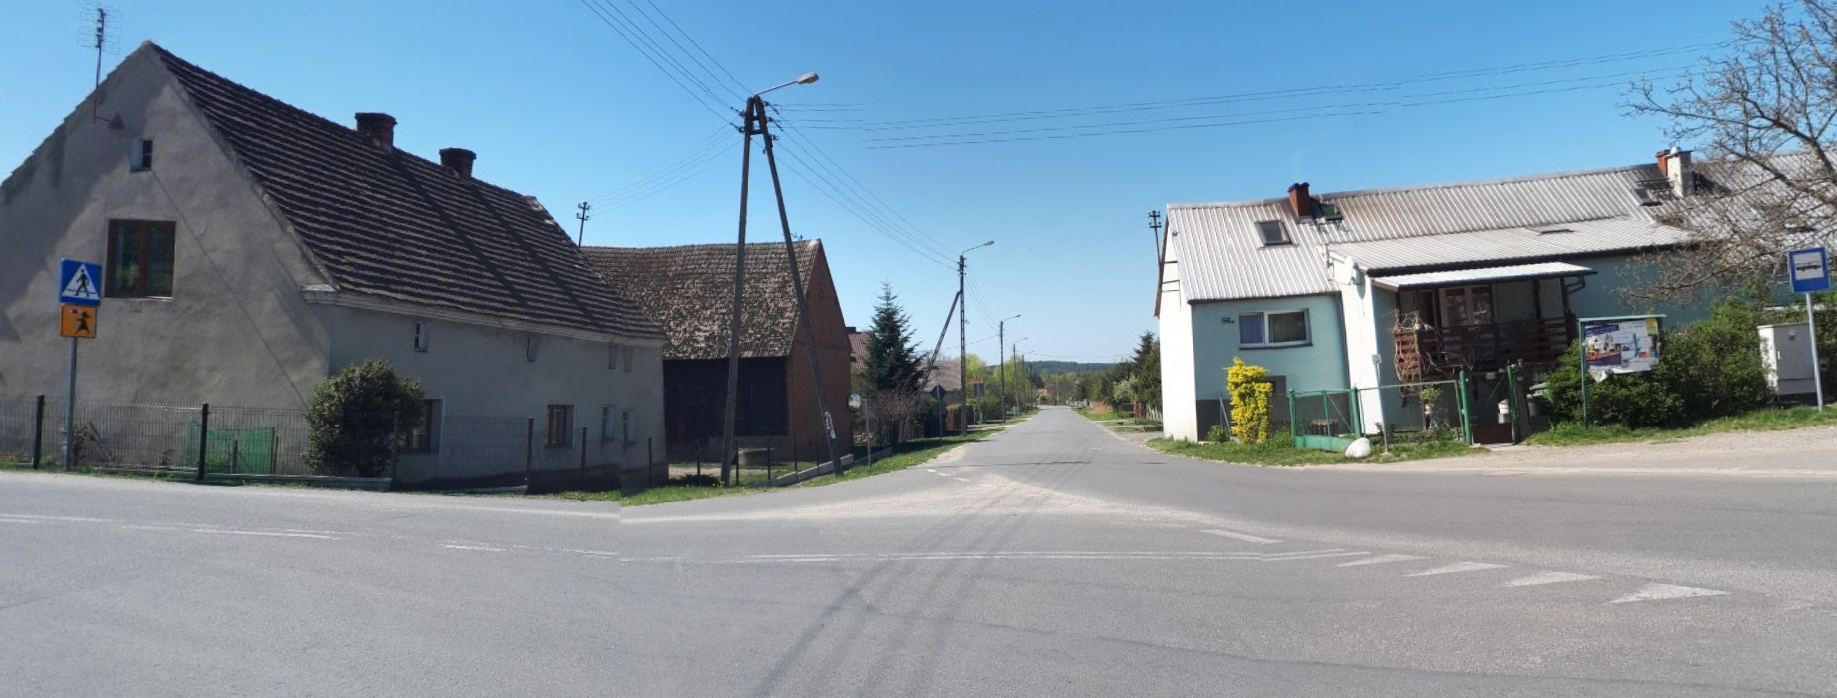
\includegraphics[width=\textwidth]{grabowno_intro.png}}
			\caption{Grabowno Wielkie}
			\label{fig:grabowno_intro}
		\end{figure}
		\begin{figure}[h!]
			\makebox[\textwidth]{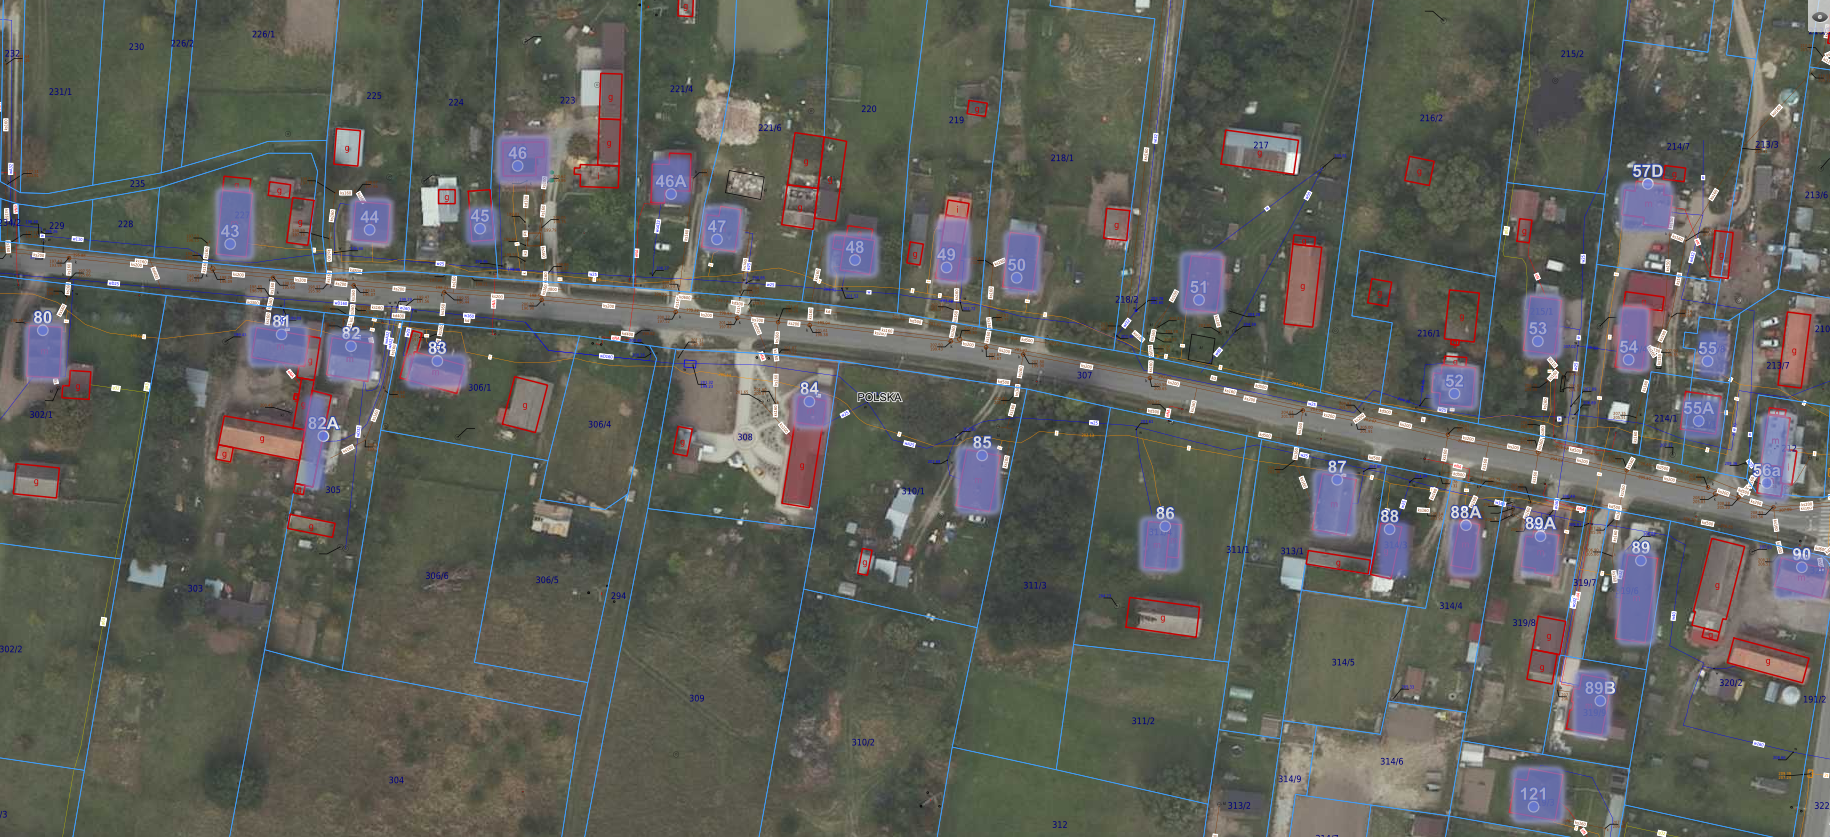
\includegraphics[width=\textwidth]{plan_intro.png}}
			\caption{Plan wsi}
			\label{fig:plan_intro}
		\end{figure}
	\end{center}

	Numery działek mające zostać objęte siecią:
	\begin{itemize}
		\item od północnej strony ulicy numery od 43 do 57
		\item od południowej strony numery od 80 do 90
	\end{itemize}